\documentclass[12pt,oneside]{article}
\usepackage[utf8]{inputenc}
\usepackage[a4paper,width=165mm,top=20mm,bottom=20mm,bindingoffset=6mm]{geometry}
% For spacing:
\usepackage{setspace}
\onehalfspacing
% To insert the last page:
\usepackage{lastpage}
% To place things more precise:
\usepackage{float} 
% To be able to insert images:
\usepackage{graphicx}
\graphicspath{ {./images/} }
\usepackage[export]{adjustbox}
% To make header and footer:
\usepackage{fancyhdr}
\setlength{\headheight}{24pt}
\pagestyle{fancy}
\fancyhead[L]{27051 Diversity and application of microorganisms}
\fancyhead[R]{
\includegraphics[height=0.68cm]{Figures/DTU.png}}
\fancyfoot[L]{Cecille, Lasse, Mathilde, Mille \& Nicolai}
\fancyfoot[C]{}
\fancyfoot[R]{Page \thepage \hspace{0.03cm} of \pageref{LastPage}}
\renewcommand{\headrulewidth}{0.1 pt}


\title{Biodiversitet - projekt}
\author{Cecille, Lasse, Mathilde, Mille \& Nicolai}
\date{March 2022}

\begin{document}

\begin{titlepage}
    \begin{center}
    
        \begin{figure}
            
\includegraphics[width=0.07\textwidth, right]{Figures/DTU.png}
        \end{figure}
    
        \Large
        27051 Diversity and application of microorganisms\\
        
        Group project
        
        \vspace{0.5 cm}
        
        \LARGE
        \rule{\textwidth}{1pt} 
        
        \textbf{\textit{Pseudomonas aruginosa}'s zinc dependent virulence factors and novel treatments}\\
        
        \Large Virulence and pathogenesis\\
        \normalsize April 27th 2022
        \rule{\textwidth}{1pt} 
    
        \vspace{0.5 cm}
        
\begin{table}[h!]
\centering
\begin{tabular}{|l|l|l|}
\hline
\textbf{Name }                          & \textbf{Study number} & \textbf{Contribution (specific section)} \\ \hline
Cecille Jasmin Elizabeth Hobbs & s203542      & 1, 2, 4.1                     \\ \hline
Lasse Schnell Danielsen        & s203512      & 1, 2, 3.0, 3.1                  \\ \hline
Mathilde Dam-Mikkelsen         & s203571      & 1, 2, 3.2                    \\ \hline
Mille Rask Sander              & s203556      & 1, 2, 4.0, 4.2                 \\ \hline
Nicolai Flohr Rimaas           & s203513      & 1, 2, 5, 6                     \\ \hline
\end{tabular}
\end{table}
        \vspace{0.8 cm}
        \begin{figure}[h!]
            \centering
            
\includegraphics[width=0.9\textwidth]{Figures/Picture 1.jpg}
        \end{figure}
        \textbf{Teachers}\\
        Lone Gram \& Mikkel Bentzon-Tilia\\ 
        \textbf{Teaching assistant}\\
        Line Roager
        \vfill
    \end{center}  
\end{titlepage}
\newpage

\tableofcontents
\newpage

\section{Summary}
In this project two virulence factors of the gram-negative bacteria \textit{Pseudomonas aeruginosa} will be presented. These are relevant as \textit{P. aeruginosa} is an opportunistic pathogen and its infections can be lethal. The two virulence factors discussed in this project includes the biofilm formation and a specific efflux pump. These two virulence factors are both to a point zinc dependent. The efflux pump is directly zinc dependent, whereas the biofilm formation depends on zinc through various factors such as the flagella construction. 

Maintaining zinc homeostasis is important for the survival of \textit{P. aeruginosa}. This makes the bacterium able to survive high and low zinc concentrations present during infection. Further it triggers the inhibition of an specific operon (\textit{oprD}), which is responsible for the influx of carbapenems. 

Biofilm formation in itself is hard to treat as it is almost impossible to penetrate with antibiotics. This is due to the biofilm matrix consisting of EPS's. Further, quorum sensing helps initiate biofilm formation. 

As antibiotics is not an efficient option on its own, alternative treatments will be discussed. These alternative treatments includes targeting of the zinc homeostasis, Photodynamic, Photothermal, and Phage Therapy. Although none of these treatments are ready for clinical trials. 

In conclusion \textit{P. aeruginosa} itself and the alternative treatments must be further researched, as there are no final solutions yet. This is partly due to the differences in research and clinical trials. 


\section{Background and purpose}
\textit{P. aeruginosa} is a gram-negative opportunistic pathogen, which is commonly found in a variety of different places such as soil and water \cite{Chatterjee2017EnvironmentalAeruginosa}.
Its large genome makes it able to host a wide range of genes for the adaptation to live under different conditions. It can be found both in its planktonic state and in its biofilm producing state. Biofilm formation can happen on both biotic surfaces and abiotic surfaces \cite{Laborda2021PseudomonasOrigin}. 
Especially on medical devices \textit{P. aeruginosa} contamination can cause serious problems as it can cause nosocomial infections. This problem is further propelled by the fact that \textit{P. aeruginosa} can survive for long stretches of time on very dry places, and sometimes even survive alcohol disinfection as reviewed in Pachori \textit{et. al} \cite{Pachori2019EmergenceReview}\cite{Laborda2021PseudomonasOrigin}.
\textit{P. aeruginosa} mainly infects patients who are immunocompromised such as cystic fibrosis patients. It was estimated that in 2017 32,600 people in the US where infected with \textit{P. aeruginosa}, and around 2,700 died from the infection \cite{MULTIDRUG-RESISTANTAERUGINOSA}. Infection with \textit{P. aeruginosa} are often extremely hard to treat, as the bacteria is resistant to the most commonly and widespread treatments options such as antibiotics \cite{Laborda2021PseudomonasOrigin}. 
Two of the major factors for \textit{P. aeruginosa}'s antibiotic resistance, are biofilm and various efflux pumps \cite{Laborda2021PseudomonasOrigin}. The efflux system, which is a series of membrane bound proteins, can export molecules from inside the cell to outside. This can enable the cell to export anti-microbial compounds from inside cell, thereby increasing resistance \cite{Perron2004CzcR-CzcSAeruginosa}. 
 
Biofilm on the other hand also promotes antibiotic resistance, but by blocking antibiotic access to the cells. Furthermore, the biofilm can support communities of bacteria, which in turn could harbor other pathogenic bacteria. These communities can also act as hot spots for gene transfer, thereby forwarding antibiotic resistance genes to other species, further complicating the challenges antibiotic resistance pose \cite{Madigan2022BrockMicroorganisms}.

Based on these factors \textit{P. aeruginosa} has been listed by the World Health Organization (WHO) as one of the most life-threatening pathogenic bacteria\cite{PRIORITIZATIONTUBERCULOSIS}. It is therefore highly relevant to find possible non-antibiotic treatments for \textit{P. aeruginosa} infections.\\ 
The purpose of this paper is to describe novel ways of treating \textit{P. aeruginosa} infections without the use of antibiotics. To do this the project will focus on \textit{P. aeruginosa}'s systems for maintaining zinc homeostasis. They are relevant since 1) they make it possible for \textit{P. aeruginosa} to survive both low- and high zinc concentration which can be present during infection 2) many of \textit{P. aeruginosa}'s virulence factors are zinc dependent as reviewed in \cite{Gonzalez2019PseudomonasPathogen}. By inhibiting \textit{P. aeruginosa}'s virulence factors, one could possibility decrease \textit{P. aeruginosa's} pathogenicity while minimizing the selective pressure on resistance. Furthermore the project will focus on \textit{P. aeruginosa}'s ability to form biofilm, as it is one of the key virulence factors in \textit{P. aeruginosa} infections.


%Bliver lavet overgang i Purpose. 
\section{Zinc homeostatis and efflux pumps in \textit{P. aeruginosa}}

Trace elements, such as zinc, are necessary for normal cell function, due to the fact that they are used as cofactors in many proteins \cite{Blencowe2003ZnIIProkaryotes}\cite{McCall2000FunctionMetalloenzymes}. Zinc is further used to regulate smaller molecules and potentially DNA as well \cite{Nejdl2014DNAIons} (and as reviewed by \cite{Krezel2016TheIons}). As a result, zinc is necessary for many of \textit{P. aeruginosa}’s virulence factors such as biofilm formation and swarming motility \cite{Mastropasqua2018EfficientLung}.

\subsection{\textit{P. aeruginosa} under zinc starvation}

Since zinc is necessary for both cellular and bacterial growth, the spread of pathogens can be reduced through decreasing levels of zinc (and other nutrients). This process is called nutritional immunity, and is imposed by the human immune system. Nutritional immunity, in relation to zinc, is achieved through zinc-chelation by proteins such as the metallophore calprotectin (as reviewed by \cite{Gonzalez2019PseudomonasPathogen}). This is the case in the lungs of cystic fibrosis patients infected by \textit{P. aeruginosa}. Here  high levels of calprotectin is a contributor to low levels of free zinc ions \cite{Gray2012SputumDiseases}. However \textit{P. aeruginosa} can still thrive and express zinc dependent virulence factors \cite{Mastropasqua2018EfficientLung}. \textit{P. aeruginosa} achieves this through at least three different systems, which help the pathogen maintain zinc homeostasis. These systems are as follows: 

\begin{itemize}
    \item \textit{P. aeruginosa} has a few different transport systems for the uptake of free zinc ions. One of these systems consists of three outer membrane pumps which can import zinc to the periplasmic space (PA0781, P11922, PA4837) \cite{Pederick2015ZnuAAeruginosa}. The transport of zinc in its free form, from the periplasmic space into the cytoplasm, is achieved through the known ZnuABC system and possibly the PA4063-PA4066 system \cite{Pederick2015ZnuAAeruginosa}\cite{Fiorillo2021StructureAeruginosa}. These different pumps helps increase the concentration of zinc in the cytoplasm, in relation to the outer environment.
    
    \item There is evidence for \textit{P. aeruginosa} being able to produce a metallophore which binds zinc. The chelated zinc-metallophore complex can then be transported into \textit{P. aeruginosa}. Hence \textit{P. aeruginosa} can compete with the host over the free zinc ions \cite{Mastropasqua2017GrowthMetallophore}.
    
    \item \textit{P. areugionsa} can produce paralogous proteins, that can replace other zinc dependent proteins. This will in turn increase available zinc (as reviewed by \cite{Gonzalez2019PseudomonasPathogen}). As an example, \textit{P. aeruginosa} can produce two paralogous proteins replacing two “zinc dependent” 50S ribosomal proteins. This releases a high amount of bound zinc in the bacteria, thereby increasing the concentration of available zinc \cite{Lim2013ThePf-5}.
\end{itemize}

\subsection{\textit{P. aeruginosa} under high zinc concentrations}
The former mentioned systems makes it possible for \textit{P. areugionsa} to survive zinc depleted conditions. Furthermore \textit{P. areugionsa} has the ability to survive high levels of zinc. This ability helps the bacterium with undermining the immune system as high zinc concentrations is used as a defense mechanism \cite{Botella2011MycobacterialMacrophages}. The high concentration of zinc is toxic as it causes mismetaliations in proteins. This results in inhibition of set proteins which have great effect on different essential pathways. It is know that zinc is used as signal during infection but whether not the zinc intoxication is an evolved mechanism is yet to be known \cite{McDevitt2011AZinc}. 

\textit{P. areugionsa} can survive high zinc concentrations through systems of efflux pumps. In  \textit{P. areugionsa} the efflux pump removing zinc from the cell interior is the CzcCBA pump. The CzcCBA efflux pump is a RND type efflux pump. The RND type efflux pumps consist of a proton antiporter located in the cytoplasmic membrane, a membrane fusion protein located through the periplasmic space, and an outer membrane protein \cite{Perron2004CzcR-CzcSAeruginosa}. This makes it possible to move the zinc from interior to the outside of the bacteria. 
The presence of zinc induces both the transcription of the \textit{czcCBA} operon and the regulatory genes \textit{czcR} \& \textit{czcS}. This makes it even harder to treat infections with \textit{P. aeruginosa} as they are dependent on the zinc concentration. 

The regulatory gene \textit{czcR} is responsible for regulating the \textit{oprD} gene \cite{Perron2004CzcR-CzcSAeruginosa}. The \textit{oprD} gene is interesting as it codes for the protein porin generally responsible for the influx of carbapenems (beta-lactam antibiotics) in gram-negative bacteria. The CzcR protein negatively regulate the expression of \textit{oprD} can result in imipenem resistant to carbapenems. It is only the dephosphorylated CzcR that can negatively regulate the expression of \textit{oprD}. The phosphorylated CzcR is necessary for triggering the transcription of the \textit{czcCBA} operon \cite{Perron2004CzcR-CzcSAeruginosa}. Whether the CzcR is phosphorylated or not, depends on the activity of CzcS as it is a histidine kinase. Histidine kinase has involvement in the dimerization, phosphotransfer, and phosphatase activity. In \textit{P. aeruginosa} two mutations were found in CzcS resulting in the protein primarily being autophosporylated. These mutations were placed in the link between the two domains in CzcS thus lowering the phosphate activity. The aforementioned lessens the dephosphorylation of CzcR resulting in a higher transcription rate of the \textit{czcCBA} operon (figure \ref{figureefflux}). The high transcription rate makes it possible to remove the toxic amount of zinc in the bacteria \cite{Perron2004CzcR-CzcSAeruginosa}. 

\begin{figure}[H]
\centering
    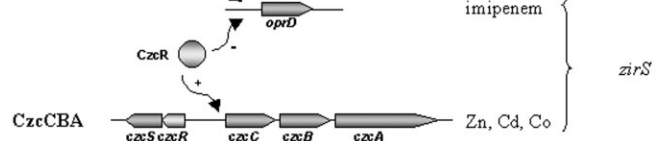
\includegraphics[width=0.80\textwidth]{Figures/Efflux figure.png}
    \caption{\footnotesize{The two operons is seen on the left hand side, where the \textit{oprD} operon is at the top and the \textit{czcCBA} operon at the bottom. When the \textit{oprD} operon is negatively regulated by CzcR the impenem antibiotic resistance is achieved. The possible regulation of the \textit{oprD} operon and the \textit{CzCBA} operon by CzcR protein is shown in middle \cite{Perron2004CzcR-CzcSAeruginosa}.}}
    \label{figureefflux}
\end{figure}

\noindent All of these tools make \textit{P. aeruginosa} able to thrive and express virulence factors under zinc starvation and in excess of zinc. Another virulence factor of \textit{P. aeruginosa} is the zinc dependent biofilm production which will be further discussed in the next section.


\section{Biofilm as a virulence factor produced by \textit{P. aeruginosa}}

The biofilm \textit{P. aeruginosa} excretes, contains specific polysaccharides as well as protein and eDNA. The biofilm formation increases the bacteria's pathogenicity by blocking the antibiotics from reaching the bacteria \cite{Thi2020PseudomonasBiofilms}. Generally biofilm can be produced both by a single bacterial species as well as by a mixture of species. This can further increase the complexity of biofilms. 

Before production of biofilm, \textit{P. aeruginosa} uses the flagella for motility in the plaktonic state until it reaches a desired surface. The construction of this flagella in \textit{P. aeruginosa} is zinc dependent due to the Zur-locus \cite{Mastropasqua2018EfficientLung}. The Zur-locus is a regulatory transcription gen, consisting of \textit{zrmA}, \textit{dksA2} and \textit{rpmE2}. When \textit{P. aeruginosa} is exposed to low levels of zinc, there is a higher expression of this locus \cite{Mastropasqua2018EfficientLung}. The genes in the Zur-locus have been related to the interference and formation of biofilm, due to the zinc dependent flagella. \textit{P. aeruginosa}'s swarming and flagella are dependent on zinc concentration. Therefore, zinc is a key player in the pre-stage of biofilm production \cite{Mastropasqua2018EfficientLung}.

\subsection{Biofilm formation} 
\noindent When biofilm is initiated, planktonic bacteria adhere to a surface which is often nutrient rich and favorable for bacterial growth. In \textit{P. aeruginosa} the attachment is mediated by the flagella or pili \cite{Ma2009AssemblyMatrix}. After adhesion the flagella and pili functions are reduced. The next stage of the biofilm formation is colonization. 
During colonization the bacteria multiply and start to produce sticky extracellular polymer substances (EPS). Throughout development the bacteria in the biofilm begin to change their metabolism which can result in complex systems. In these complex systems the bacteria at the top of the biofilm can be different from those at the base. Further the complex systems in \textit{P. aeruginosa} biofilm can take form of mushroomlike columns and channels. Finally the mature biofilm disperses allowing the detached bacteria to colonize to new locations \cite{Ma2009AssemblyMatrix} (figure \ref{fig:biofilm}). \\

\begin{figure}[H]
    \centering
    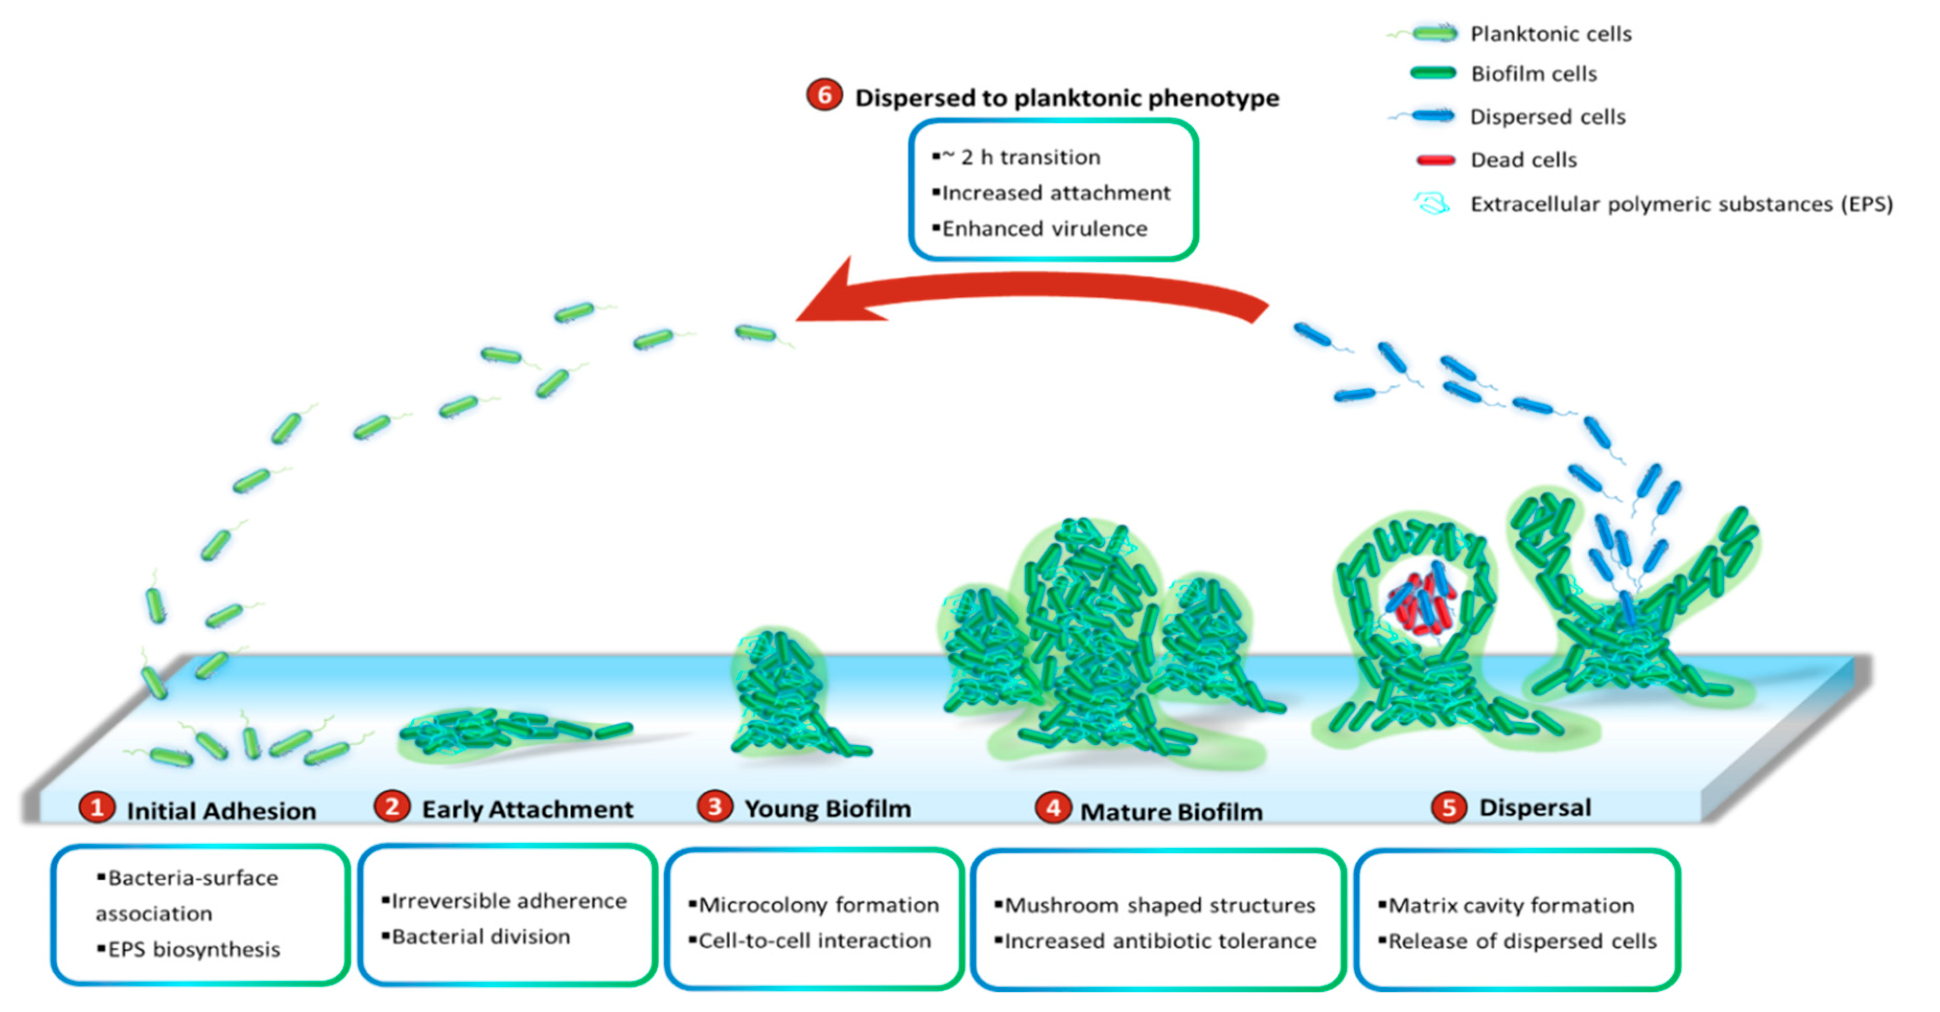
\includegraphics[width=\textwidth]{Figures/Screenshot 2022-04-27 at 10.00.54.png}
    \caption{\footnotesize{The cycle of \textit{P. aeruginosa} biofilm formation. The cycle is divided into six stages. The first step is initial adhesion, followed by early attachment. During these first stages the bacteria begin to produce extracellular polymeric substances followed by cell division. The following steps are the formation of microcolonies and the further development of these microcolonies into mushroom-shaped structures. Finally the mature biofilm disperses bacteria which allows for new colonization sites \cite{Thi2020PseudomonasBiofilms}.}}
    \label{fig:biofilm}
\end{figure}

\subsection{Quorum sensing as a factor in biofilm formation}

\noindent Inside the biofilm, nutrients can fluctuate between the bacteria. Further the matrix creates an environment for natural transformation and gen exchange, as well as resistance against the outside environment \cite{Madigan2022BrockMicroorganisms}. Bacteria inside the biofilm are tightly packed, which allows cell-to-cell communication called quorum sensing (QS). The phenomenon of QS is mainly found among gram-negative bacteria, and it works through regulatory molecules called autoinducers. Autoinducers can diffuse and be absorbed between bacteria within the biofilm. Specifically for \textit{P. aeruginosa}, high expression of the autoinducer acyl homoserine lactones (AHL), binds and activates transcriptional proteins \cite{Madigan2022BrockMicroorganisms}. The formation of biofilm is controlled by autoinducers as well as the concentration of secondary messengers, such as cyclic di-guanosine monophosphate (c-di-GMP). \\

\noindent When the population of \textit{P. aeruginosa} reaches a high enough concentration of AHL, secondary messengers related to biofilm formation can be expressed. One of these is secondary messengers is c-di-GMP. An increase in c-di-GMP levels cause weakend function of the flagellum as well as the fabrication of EPSs \cite{Colvin2012TheMatrix} \cite{Madigan2022BrockMicroorganisms}. Part of these EPSs is the pentasaccharide Psl which shields the biofilm bacteria from antimicrobials \cite{Billings2013TheBiofilms}. Additionally Psl functions as a signaling molecule for the production of c-di-GMP. Elevated c-di-GMP levels also creates a thicker and more robust biofilm \cite{Irie2012Self-producedAeruginosa/i}. Furthermore lysed cells excrete DNA that can also contribute to the biofilm formation.\\

\noindent Biofilm is a major problem for patients with cystic fibrosis as the matrix makes it difficult to treat. During hypoxic and anoxic conditions \textit{P. aeruginosa} has indicated the ability to grow slowly as unattached cell aggregates, reviewed in Thi \textit{et. al.} \cite{Thi2020PseudomonasBiofilms}. Slowly growing biofilms with limited oxygen are ascribed to antibiotic recalcitrance \cite{Thi2020PseudomonasBiofilms}. Still to this day, there hasn't been found an effective treatment to fight the invasion of biofilm, when infected with \textit{P. aeruginosa}. Alternative treatment options to antibiotics will be discussed in the following section. 





\section{Alternative treatment options for \emph{P. aeruginosa} infections} \label{Alternative treatment}

Due to increasing antibiotic resistance in \emph{P. aeruginosa} strains, novel methods of dealing with the pathogen are needed. Two of the most significant contributors to the antibiotic resistance is the formation of biofilm, which can block external compounds, as well as the efflux system. Therefore methods targeting biofilm formation or the zinc homeostasis could be speculated as alternatives to antibiotics. 

\subsection{Targeting zinc homeostasis}
Biofilm formation could be targeted indirectly by inhibiting the systems maintaining zinc homeostasis. This would lower \emph{P. aeruginosas} pathogenicity, since swimming and swarming motility depend on the flagella, which in turns depends on free zinc ions. An example of this was demonstrated by Mastropasqua \emph{et. al} \cite{Mastropasqua2018EfficientLung}. They proved the flagella synthesis is negatively regulated by low zinc concentrations. This in turns impaired the swarming mobility for \emph{P. aeruginosa}, which would decrease the pathogenicity \cite{Mastropasqua2018EfficientLung}.\\

\noindent A challenge posed by inhibiting the zinc homeostasis, could be the large amount of regulatory systems for the import of zinc. Here one inhibited system might just be replaced by the up-regulation of another one.

Another way of targeting the zinc homeostasis, is by the zinc uptake pathway. Since permeability of zinc in the biofilm is low, the bacteria uses metallophores as chelating agents to transport zinc into the cells. This opens a possibility to bio-engineer metallophores to carry antimicrobials instead of zinc. These bio-engineered compounds can be applied to biofilm, to carry antimicrobial agents straight into the cell \cite{Mastropasqua2018EfficientLung}.

\subsection{Photodynamic therapy}
Another promising approach to dealing with bacterial biofilm, is the use of Photodynamic Therapy (PDT). The basis of PDT, is using non-toxic photosensitizers (PS) which are light sensitive compounds. When the PS are illuminated with visible light, it reacts with oxygen and creates reactive oxygen species (ROS) \cite{Darabpour2016ChitosanStudy}. ROS can act on a myriad of targets spanning from biofilm matrices, cell membranes, cellular organelles as well as macromolecules \cite{Darabpour2016ChitosanStudy}. Different ROS can also be very specific in which targets they interact with, thus making them ideal for treatment options. Furthermore, the ROS can be immobilized onto nanoparticles which can improve drug delivery into biofilm \cite{Darabpour2016ChitosanStudy}. An advantage to PDT is the unlikeliness for bacteria to evolve resistance. This is due to the PS not needing to enter the cell to cause damage. Therefore cells can't block the uptake or increase detoxification \cite{Tavares2010AntimicrobialTreatment}.

\subsection{Photothermal therapy}           
In Photothermal Therapy (PTT), light is again utilized to combat bacterial infections, but in a different way. In PTT near infrared light is emitted at nanomaterials, which creates extreme localized heat zones that causes damage to the biofilm. Different nanomaterials can be used for this, ranging from carbon based to gold or silver particles \cite{Korupalli2017Acidity-triggeredInfection}. This type of treatment was demonstrated by Al-Bakri \emph{et. al}, who used gold nanorods (AuNR) and phospholipid-polyethylene (PEG). This resulted in a $\sim$6 log cycle reduction in viable count compared to the reference \cite{Al-Bakri2019Photothermal-inducedBiofilm}. This method also has the possibility to be combined with phage therapy.

\subsection{Phage therapy}
In phage therapy, bacteriophages are used to infect and lyse cells. The main advantage of using phages is their specificity for particular bacterial species. Although bacteria can become resistant to phages, this often entails  a trade-off between the cells. This trade-off cause the cells to lose their antibiotic resistance \cite{Chan2018PhageAeruginosa}. This is partly because their lyseing mechanism is distinct from those of antibiotics \cite{Chan2018PhageAeruginosa}. To increase efficiency of treatment, phage therapy can be combined with PTT. This however is still experimental, and isn't seen in clinical trials. 




\section{Conclusion}
\emph{P. aeruginosa} is listed as a priority pathogen for Research and Development of new antibiotics by the World Health Organization. This is due to the antibiotic resistant phenotype shown by \emph{P. aeruginosa}, as well as the possibility of HGT of the antibiotic resistance genes to other species of bacteria. The resistance to antibiotic can be attributed to efflux pumps in the cells and biofilm formation. As mentioned previously, the biofilm is indirectly zinc dependent while some efflux pumps are directly depended.  

Zinc homeostasis is regulated in different ways, depending on whether there is a depletion or excess of zinc. If there is a depletion of zinc, the cells can acquire the metal from uptake through membrane transport proteins, metallophores, or by creating paralogous proteins. These paralogous proteins can replace zinc requiring proteins in order to free the metal. If an excess of zinc is present the efflux system is activated, where membrane proteins pump excess zinc out of the cells. 

Another virulence factor of \textit{P. aeruginosa} is the zinc dependent biofilm, which consists of polysaccharides, eDNA and proteins. The sticky matrix from the biofilm helps the bacteria attach to different surfaces, and also protects the bacteria against extrinsic stress like antibiotics. The biofilm can include multiple different species of bacteria, from where HGT can occur. This further complicate the challenge of antibiotic resistance. In biofilm communities, the cells often regulate behaviour by quorum sensing. Some genes are only expressed when larger numbers of colonies are present, to improve fitness. 

Due to the antibiotic resistant phenotype of \emph{P. aeruginosa}, other methods are being researched as alternative treatment options. As described, the zinc uptake is vital for the pathogenesis of \emph{P. aeruginosa}. Therefore, a strategy to withstand the pathogen could be by impairing the zinc uptake in bacteria. Another method is to target the metallophores which are responsible for zinc uptake. By bio-engineering them anti-microbials could be delivered straight into the cell. 

Other alternative treatment options rely on light to damage the biofilm - Photothermal and Photodynamic Therapy. Here light can either be used to create localized heat spots which can cause damage to the biofilm, or create ROS which can cause oxidative stress. These methods could also be supplemented with phage therapy. All of these treatment options are still in the development phase and not ready for commercial use. This is also due to the complexity when using them on humans as one could harm unintended cells.  



%%%%%%%%%%%%%%%%%% indsættelse af kilder %%%%%%%%%%%%%%%%%%
\addcontentsline{toc}{section}{References}
\bibliography{references.bib}
%\bibliography{FællesRef.bib}
\bibliographystyle{ieeetr}

\end{document}
